\subsection{بخش د}
در این بخش به بررسی درنظرگرفتن زاویه پیش‌بین در قانون هدایت فرمان به خط دید پرداخته شده است.
\begin{figure}[H]
	\centering
	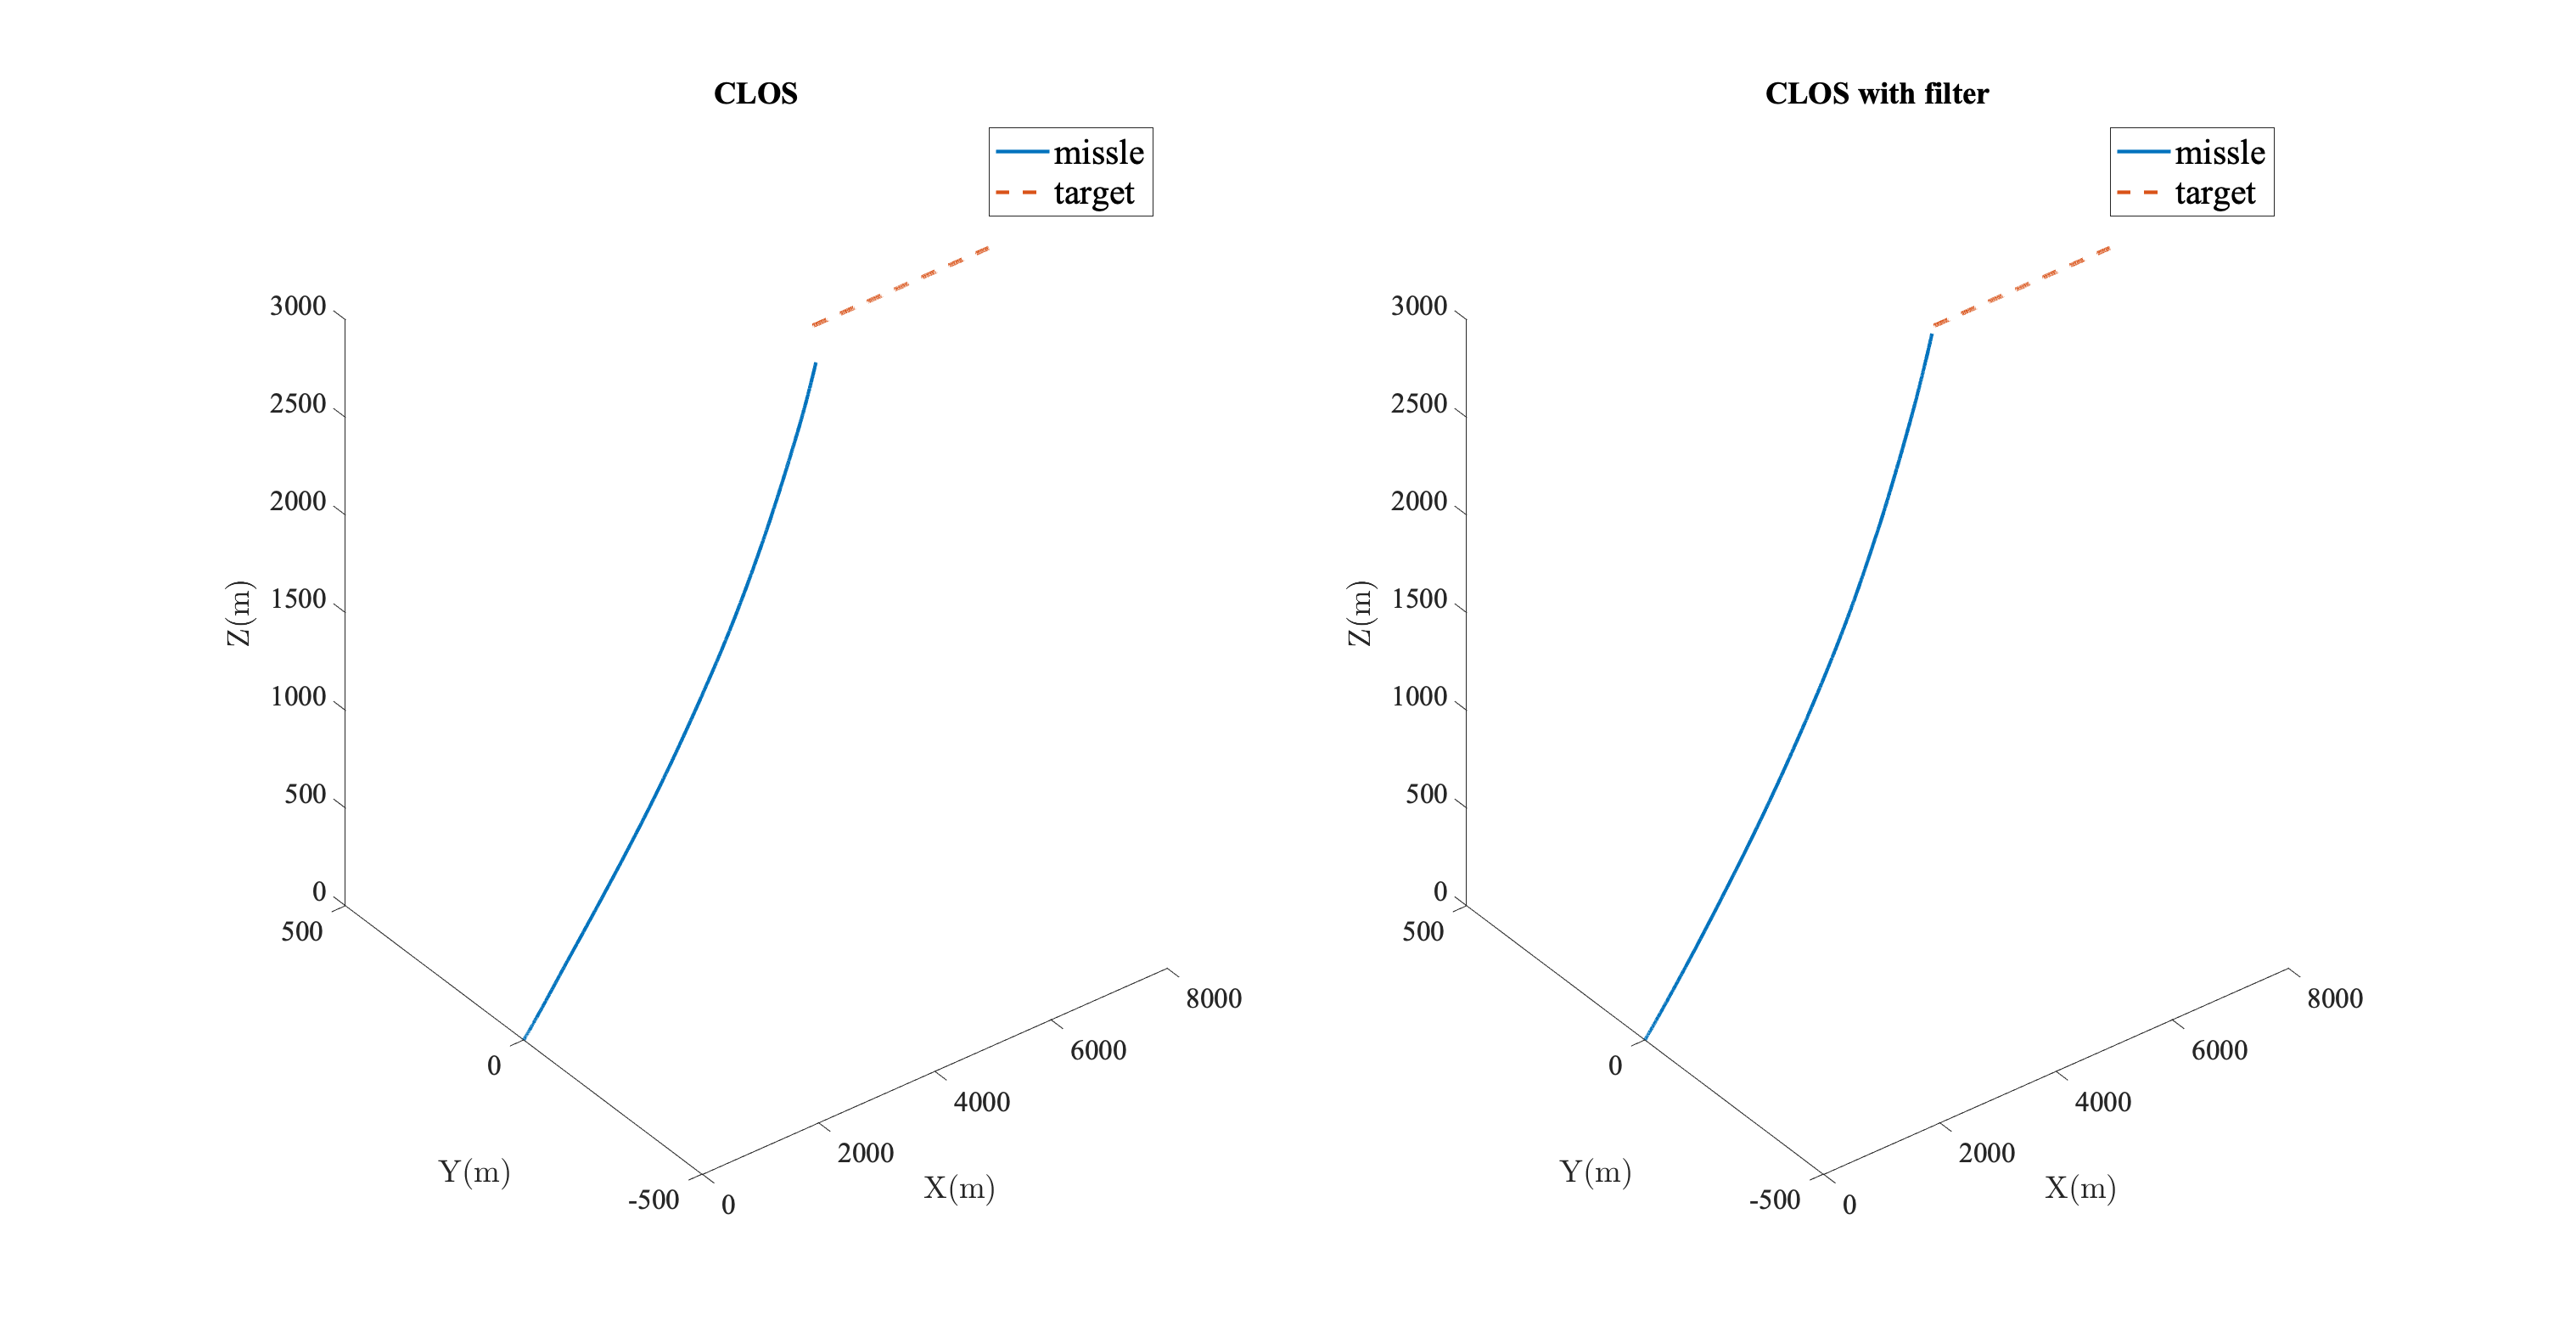
\includegraphics[width=\linewidth]{../Figure/i/3DoF_missle_vs_target_state_CLOS}
	\caption{مقایسه موقعیت موشک و هدف به صورت سه بعدی در دو نمودار  برای بررسی درنظرگرفتن زاویه پیش‌بین در قانون هدایت فرمان به خط دید}
\end{figure}


\begin{figure}[H]
	\centering
	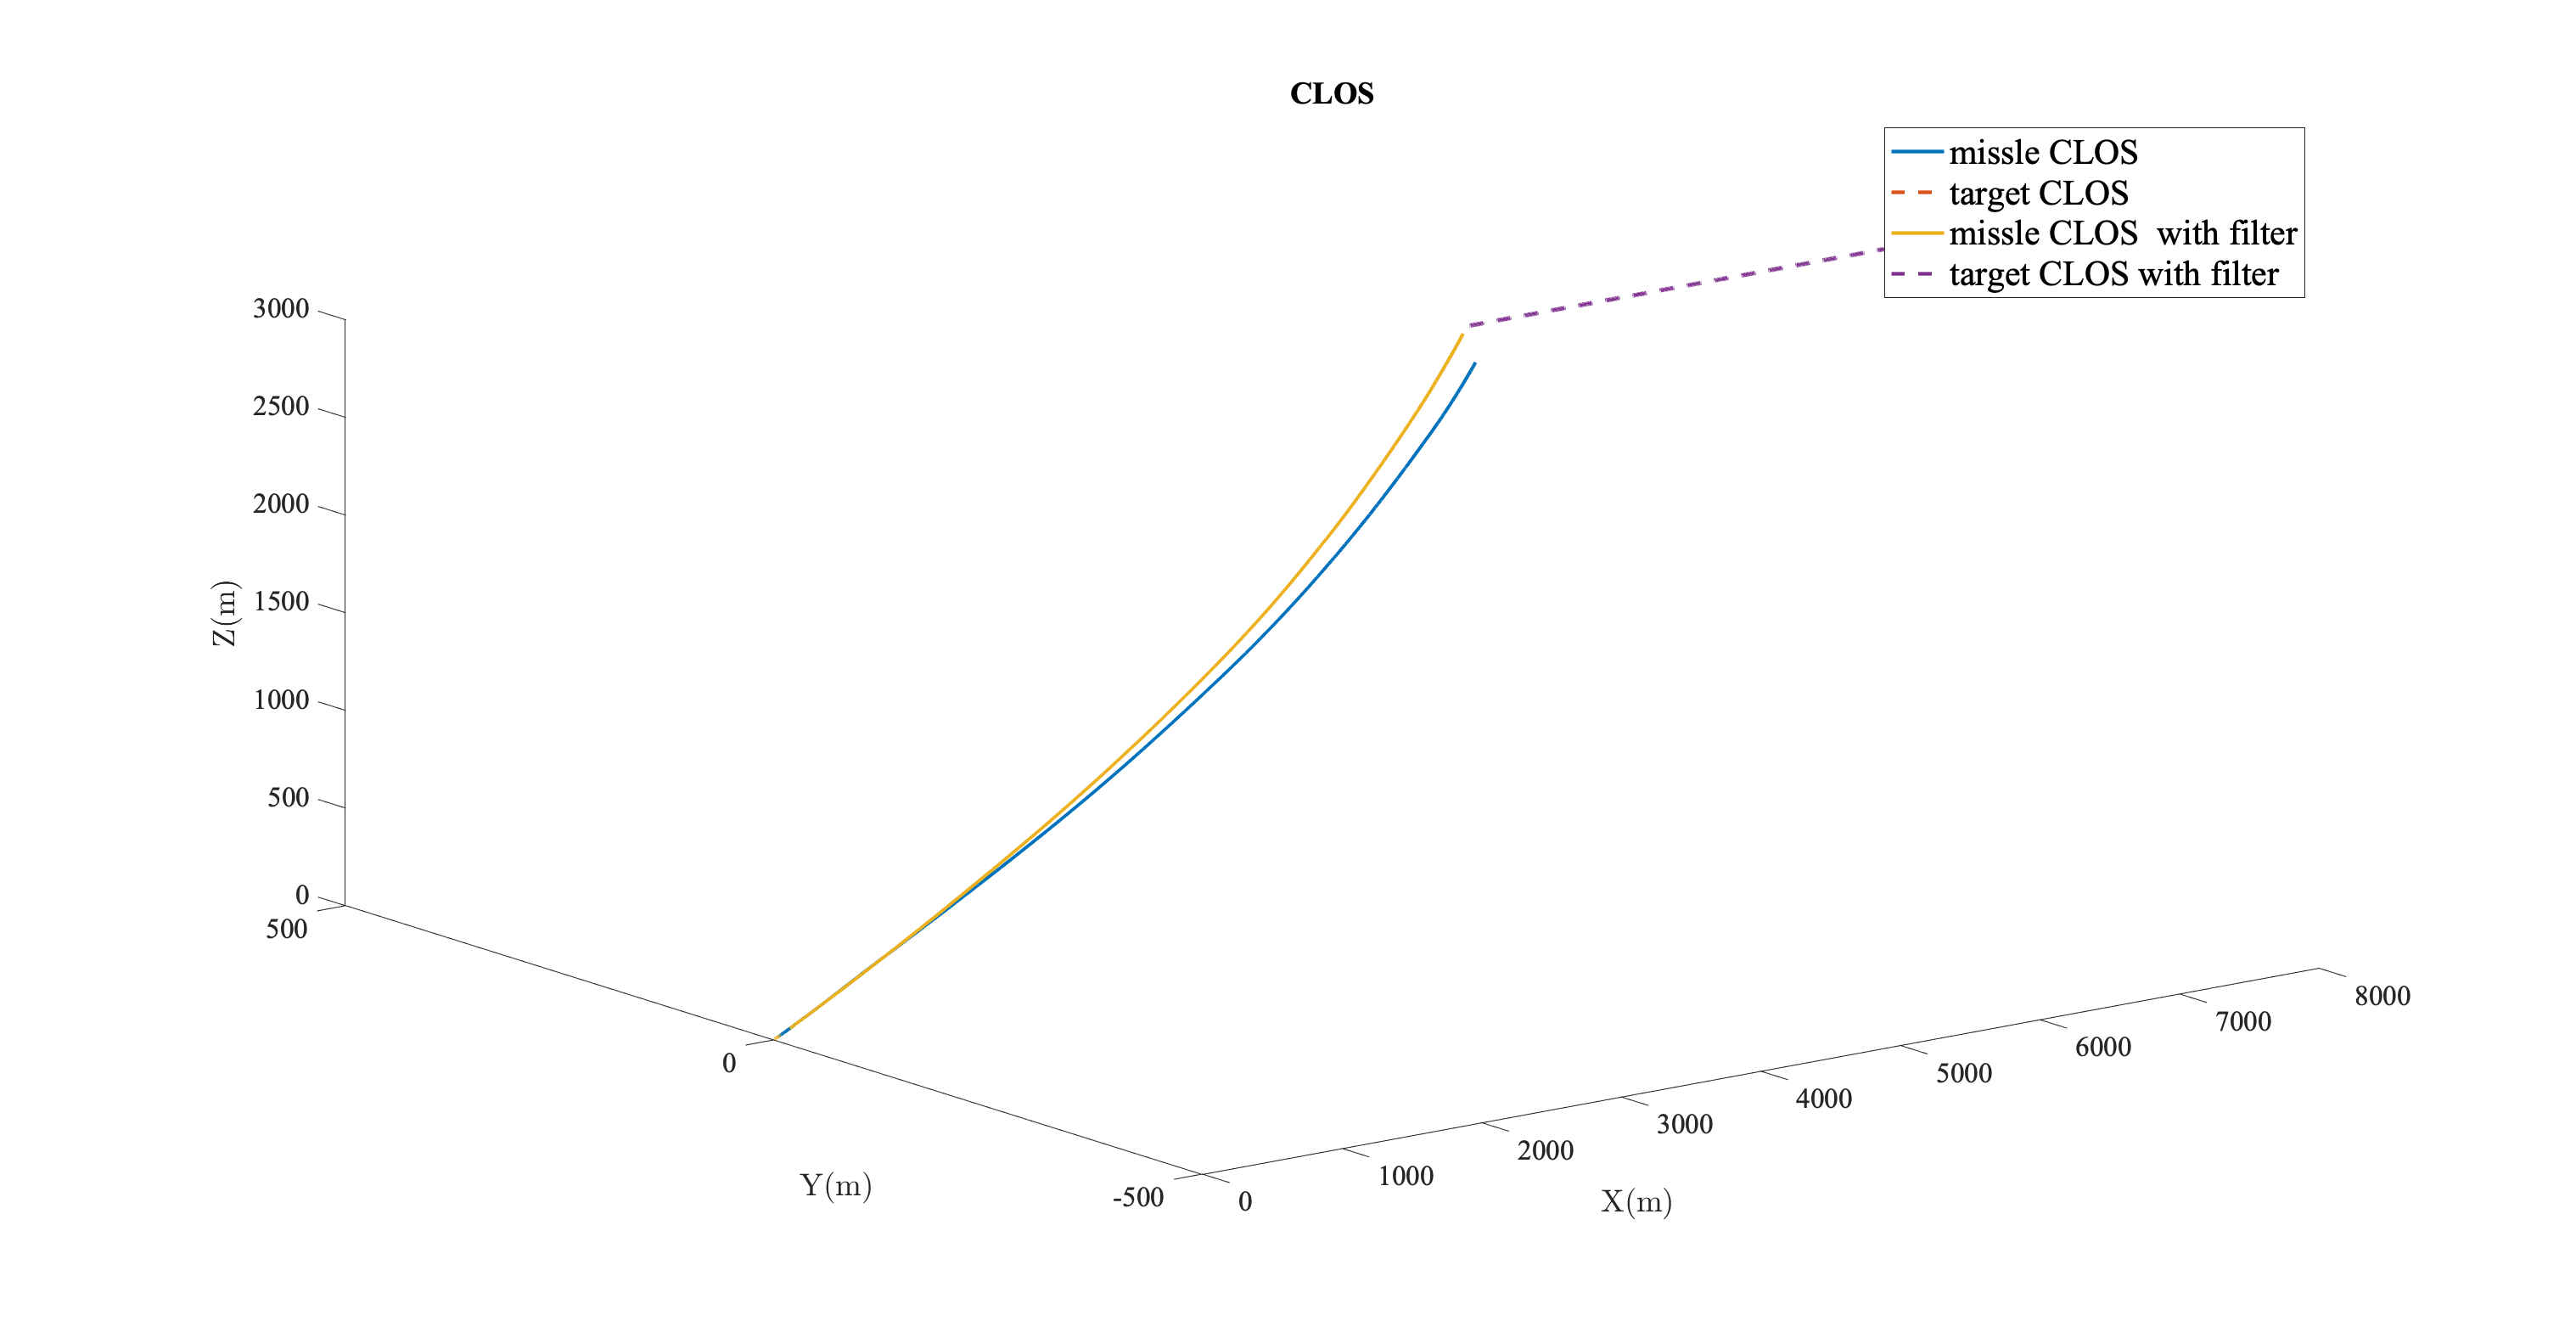
\includegraphics[width=\linewidth]{../Figure/i/3DoF_missle_vs_target_state_CLOS_all_in}
	\caption{مقایسه موقعیت موشک و هدف به صورت سه بعدی در یک نمودار برای بررسی درنظرگرفتن زاویه پیش‌بین در قانون هدایت فرمان به خط دید}
\end{figure}

\begin{figure}[H]
	\centering
	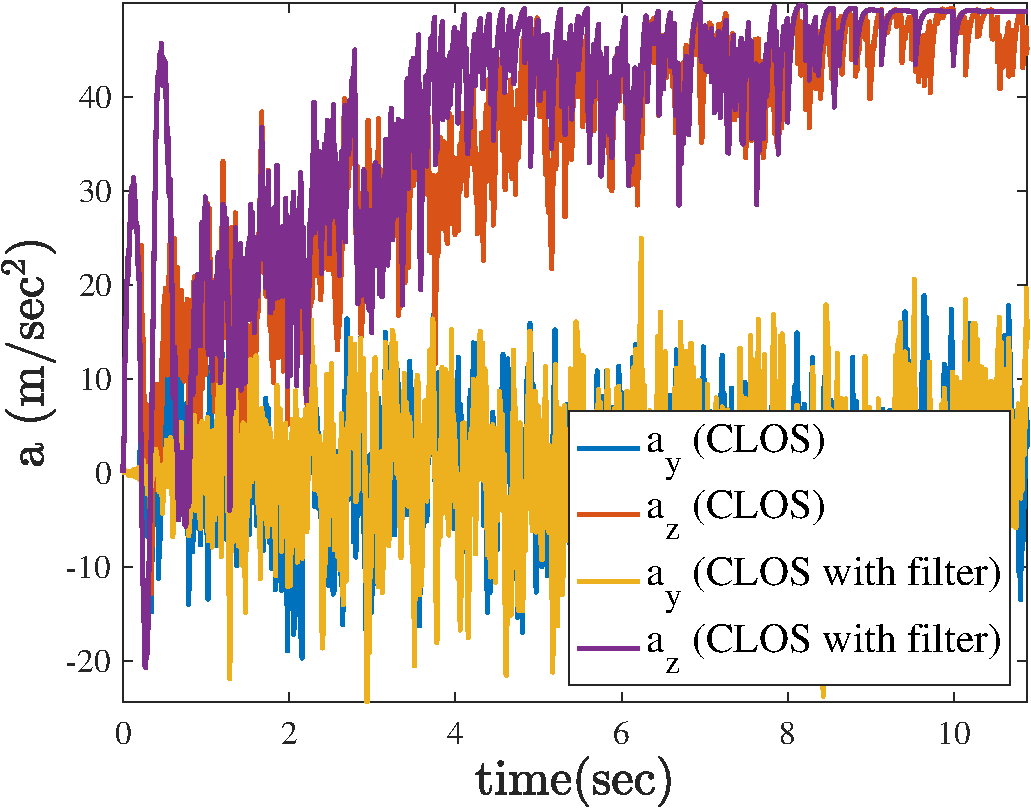
\includegraphics[width=.75\linewidth]{../Figure/i/command}
	\caption{مقایسه فرمان موشک برای بررسی درنظرگرفتن زاویه پیش‌بین در قانون هدایت فرمان به خط دید}
	
\end{figure}

\begin{figure}[H]
	\centering
	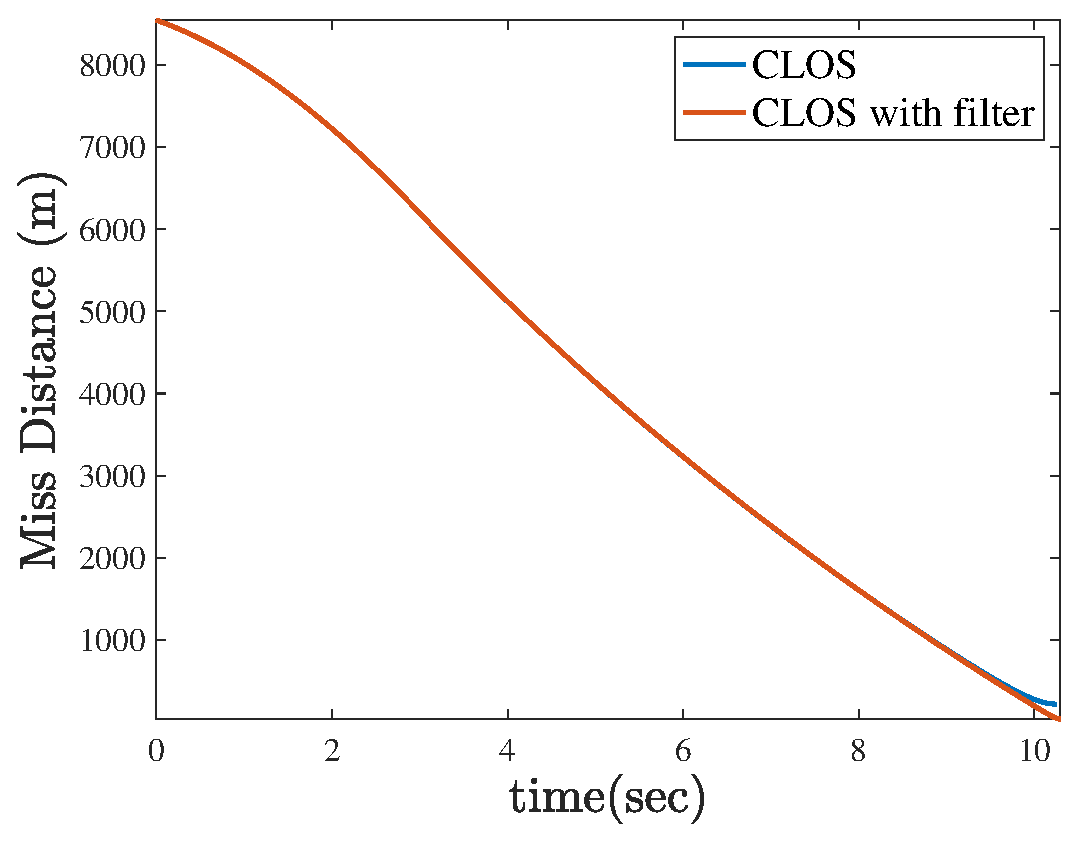
\includegraphics[width=.75\linewidth]{../Figure/i/miss_distance}
	\caption{مقایسه فاصله ازدست‌دهی موشک برای بررسی درنظرگرفتن زاویه پیش‌بین در قانون هدایت فرمان به خط دید}
\end{figure}



\begin{table}[H]
	\caption{فاصله ازدست‌دهی در قانون هدایت فرمان به خط دید}
	\centering
	\begin{tabular}{ccc}
		\hline
		\lr{Standard Deviation} & \lr{Mean} & \lr{Signal} \\
		\hline
		\lr{0.0588}  &\lr{0.4473} & \lr{$\theta$}   \\
		\lr{0.8462}  &\lr{0.0553} & \lr{$\dot\theta$}   \\
		\lr{65.5899}  &\lr{0.3548} & \lr{$\ddot\theta$}   \\
		\hline
	\end{tabular}
\end{table}